% Online Software Overview

The pixel online software is based on the xdaq toolkit and is
built from a number of different components (applications). The
different xdaq based components are shown in green in 
Fig.~\ref{fig:components}. The top level application is the 
PixelSupervisor. This application is responsible for the overall
coordination of the pixel DAQ. The PixelSupervisor talks to the
supervisors that directly control the hardware. For example 
we have the PixelFECSupervisor that provides the interface to the
pixel FECs. Similarly the PixelFEDSupervisor controls FEDs. 
In production at P5, there are multiple instances of the PixelFECSupervisor and
PixelFEDSupervisor; one per VME crate.\footnote{The strip tracker
uses a design where there is one supervisor per VME board.}

\begin{figure}
\begin{center}
 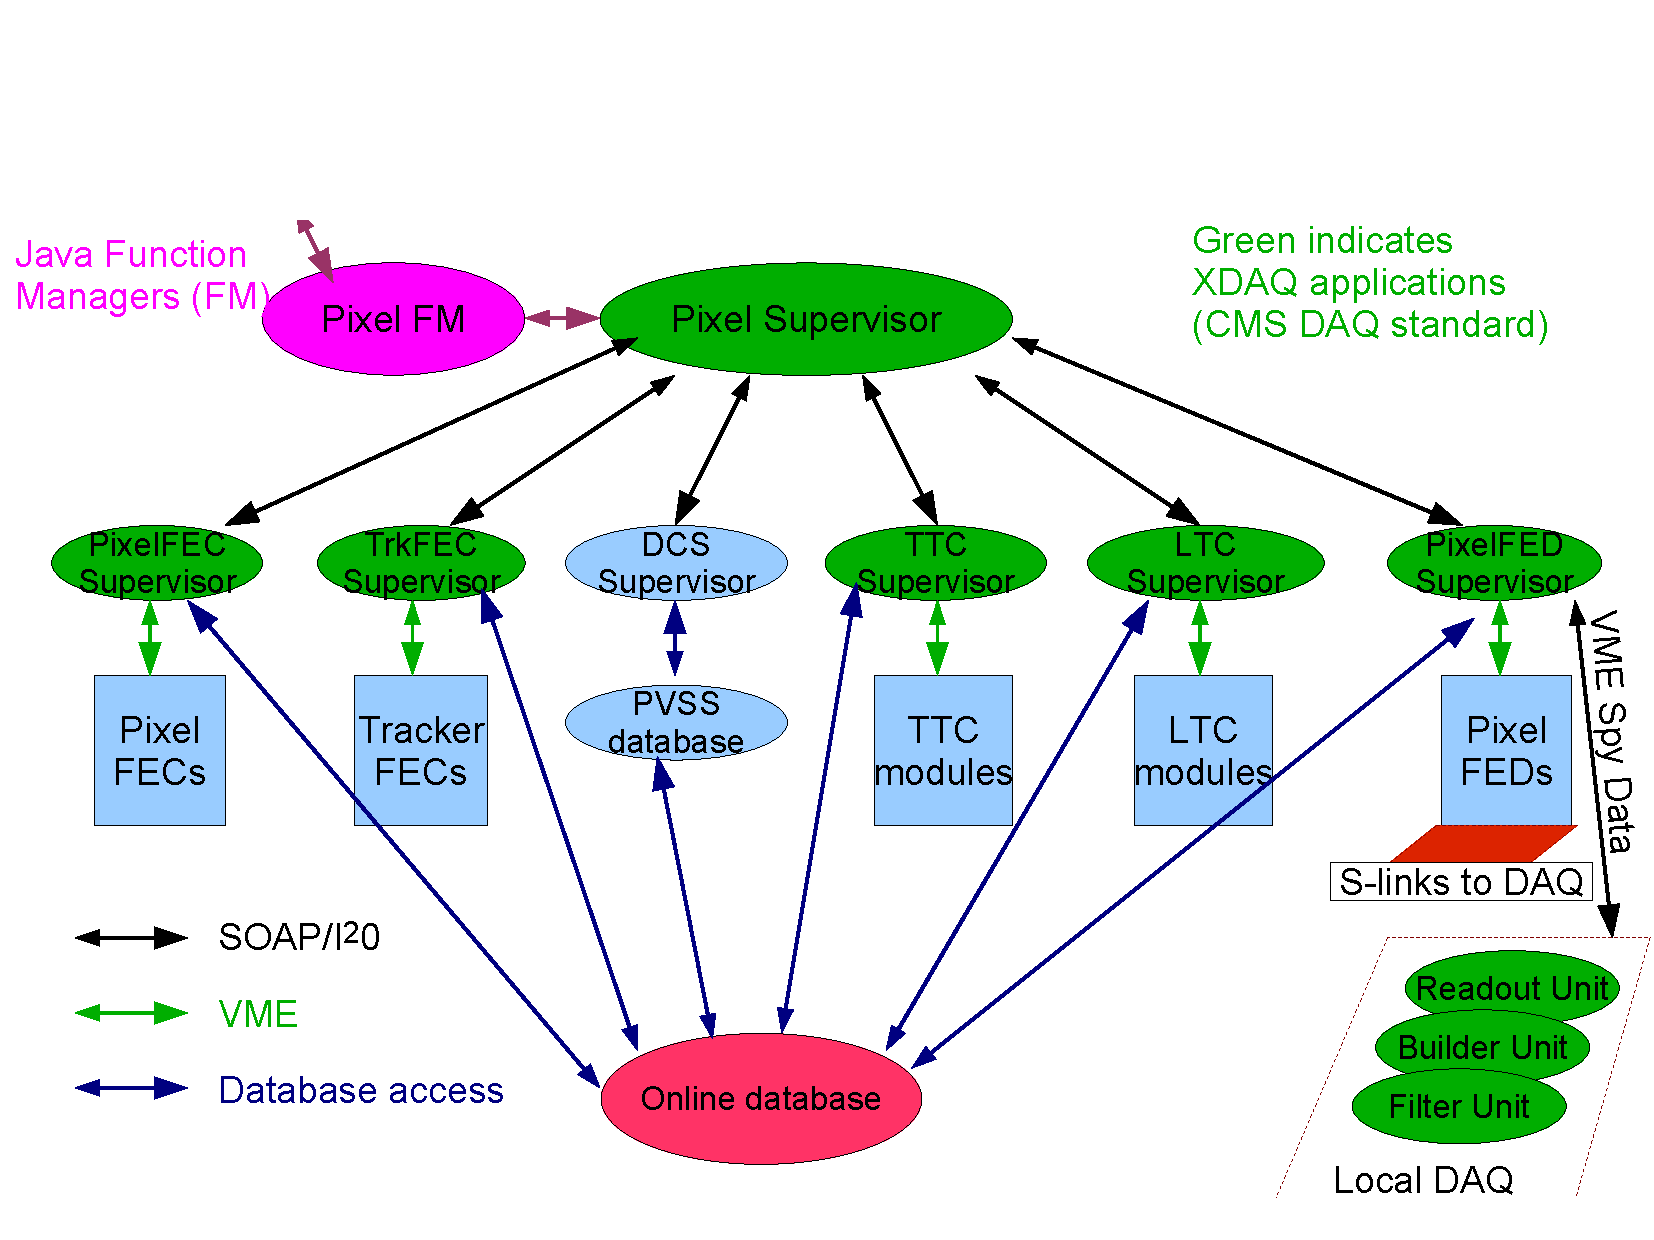
\includegraphics[width=0.99\textwidth]{POScomponents.pdf}
\end{center}
\caption{The different applications that compose the Pixel Online Software.}
\label{fig:components}
\end{figure}

The various supervisors run as indepdendent processes, or even on
different computers. Therefore, in order to communicate with each
other they must exchange messages on the network. This is done using
the SOAP protocol.

In the pixel online software the code is distributed
among a number of packages. These packages are listed
here.
\begin{itemize}
\item PixelCalibrations
%\item PixelCalibrationInterface
\item CalibFormats/SiPixelObjects
\item PixelConfigDBInterface
%\item PixelDCSSupervisor
\item PixelDCSInterface
\item PixelFECInterface
\item PixelFECSupervisor
\item PixelFEDInterface
\item PixelFEDSupervisor
\item PixelFunctionManager
\item PixelLTCSupervisor
\item PixelSupervisor
\item PixelTKFECSupervisor
\item PixelTTCSupervisor\footnote{In use through tag {\tt POS\_3\_1\_2}; deprecated starting in {\tt POS\_3\_2\_0}.}
\item PixelUtilities
\end{itemize}
The package dependency tree is shown in Fig~\ref{fig:dependencies}.
The supervisor applications are at the top and depend on the
packages below. We should make sure that the dependencies
form a tree and not contain loops. (If it seems necessary
to create a loop the solution is almost always to separate
out some piece of code into a separate package.)

\begin{figure}
\begin{center}
 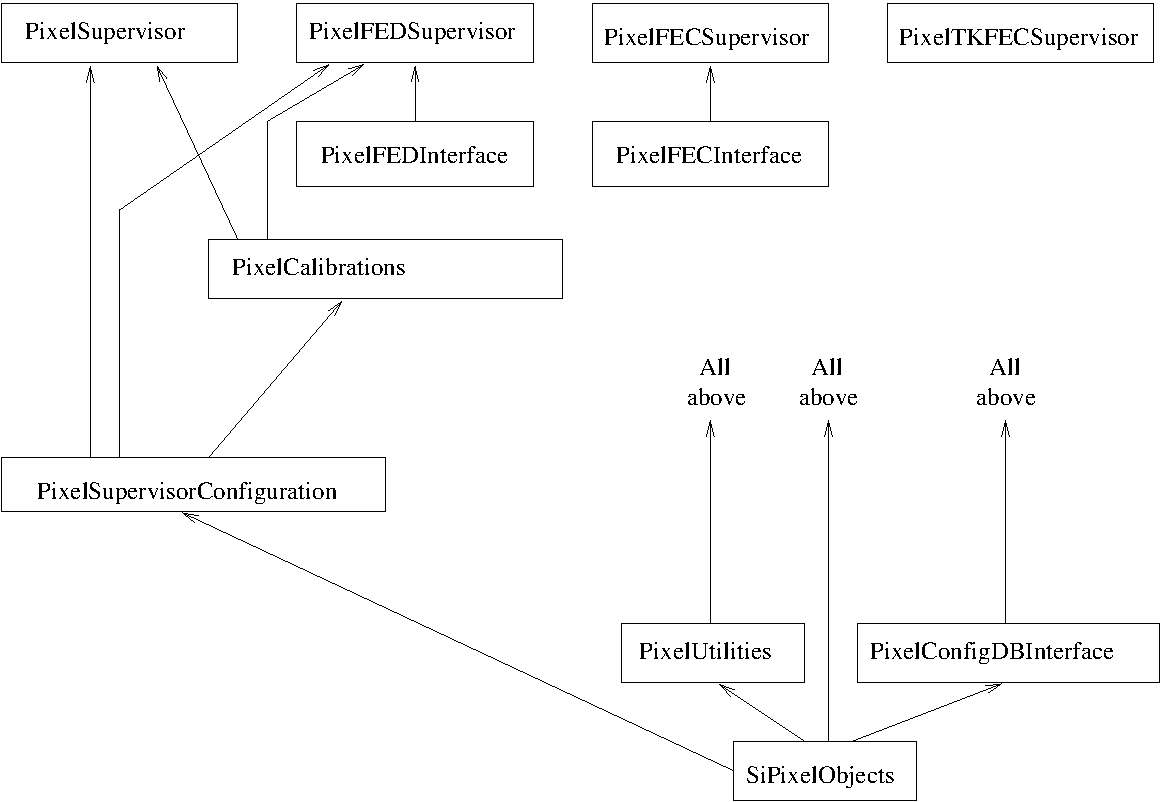
\includegraphics[width=0.99\textwidth]{package_dep.pdf}
\end{center}
\caption{The dependencies among the packages are indicated here.
At top are the supervisor applications. }
\label{fig:dependencies}
\end{figure}

\subsection{PixelSupervisor}
The PixelSupervisor is the top level xdaq application
in the pixel online software. As described above it takes
commands from the function manager. There is one pixel
supervisor for the pixel online system.

\subsubsection{Functions}
The main function of the PixelSupervisor is to coordinate the
activities of the other supervisors, particularly during configuration
(see Sec.~\ref{sec:configuration}) and calibration (see
Sec.~\ref{sect:calib}). It is responsible for updating the
configuration database with new settings obtained by calibrations.

The PixelSupervisor also communicates the state of the pixel
xdaq software (POS) to the Level 1 Function Manager (Sec.~\ref{sec:l1fm}).

\subsubsection{Interface}
The PixelSupervisor web GUI is an html page, which by default
refreshes every few seconds. It displays information about the current
configuration, or if it is not configured it allows the user to select
a possible configuration from a list and configure the detector using
that configuration.

The PixelSupervisor runs the JobControl Monitor, which is a utility
that periodically sends ``heartbeat'' SOAP messages to the JobControl
processes running on the various machines at P5. The PixelSupervisor
GUI uses the replies from these SOAP messages to display whether any of
the POS xdaq processes has crashed, or whether any of the JobControl
processes themselves are unresponsive. (Note that we typically only
run JobControl at P5, so this feature is not available elsewhere.)

\subsection{PixelFECSupervisor}
The FEC Supervisor controls the pixel FECs. This means it is
responsible for loading the configuration parameters for the ROCs from
the configuration database and programming those parameters into the
detector.

\subsection{PixelFEDSupervisor}
The FED Supervisor controls and monitors the pixel FEDs.

\subsection{PixelTKFECSupervisor}
The PixelTKFECSupervisor controls the tracker FEC hardware. The
pixel system uses the tracker FEC hardware slow I2C to
initialize the fast I2C used for the download of most 
configuration data.

\subsection{PixelTTCSupervisor}
The PixelTTCSupervisor controls the pixel TTC module used for trigger
and timing. Among other things the TTC module is used during
calibrations to generate triggers. In modern releases of the software,
the PixelTTCSupervisor has been deprecated in favor of the
TTCciControl, which is a standard package maintained by the TTC group.

\subsection{PixelLTCSupervisor}
The PixelLTCSupervisor is used for the local trigger control.

